\section{Fallbeispiel AXA Gesundheitsvorsorge}

In diesem Kapitel wird die Anwendbarkeit der künstlichen Intelligenz zur automatisierten Verarbeitung von eingereichten Rechnungen bei der AXA Gesundheitsvorsorge überprüft.

Es wird erst ein Überblick über den Prozess gewährt, aus welchem anschliessend Aufgaben abgeleitet werden, welche mit Hilfe von künstlicher Intelligenz automatisiert werden sollen.

\subsection{Einleitung}

Der Prozess der Rechnungseinreichung und -verarbeitung (vgl. Abbildung \ref{prozessaxa}) der AXA kann aufgrund zwei verschiedener Ereignisse angestossen werden. In jedem Fall reicht der Kunde eine Rechnung ein. Dies kann er entweder digital, im Kundenportal, oder per Post machen. 

\begin{figure}[h]
    \captionsetup{width=.8\linewidth}
    \caption{Prozess der Rechnungseinreichung und -verarbeitung der AXA Gesundheitsvorsorge. Vom Kunden per Post oder über das Kundenportal eingereichte Rechnungen durchlaufen mehrere Prozessschritte in Verantwortung unterschiedlicher Organisationen.}
    \label{prozessaxa}
    \centering
    \vspace{0.2cm}
    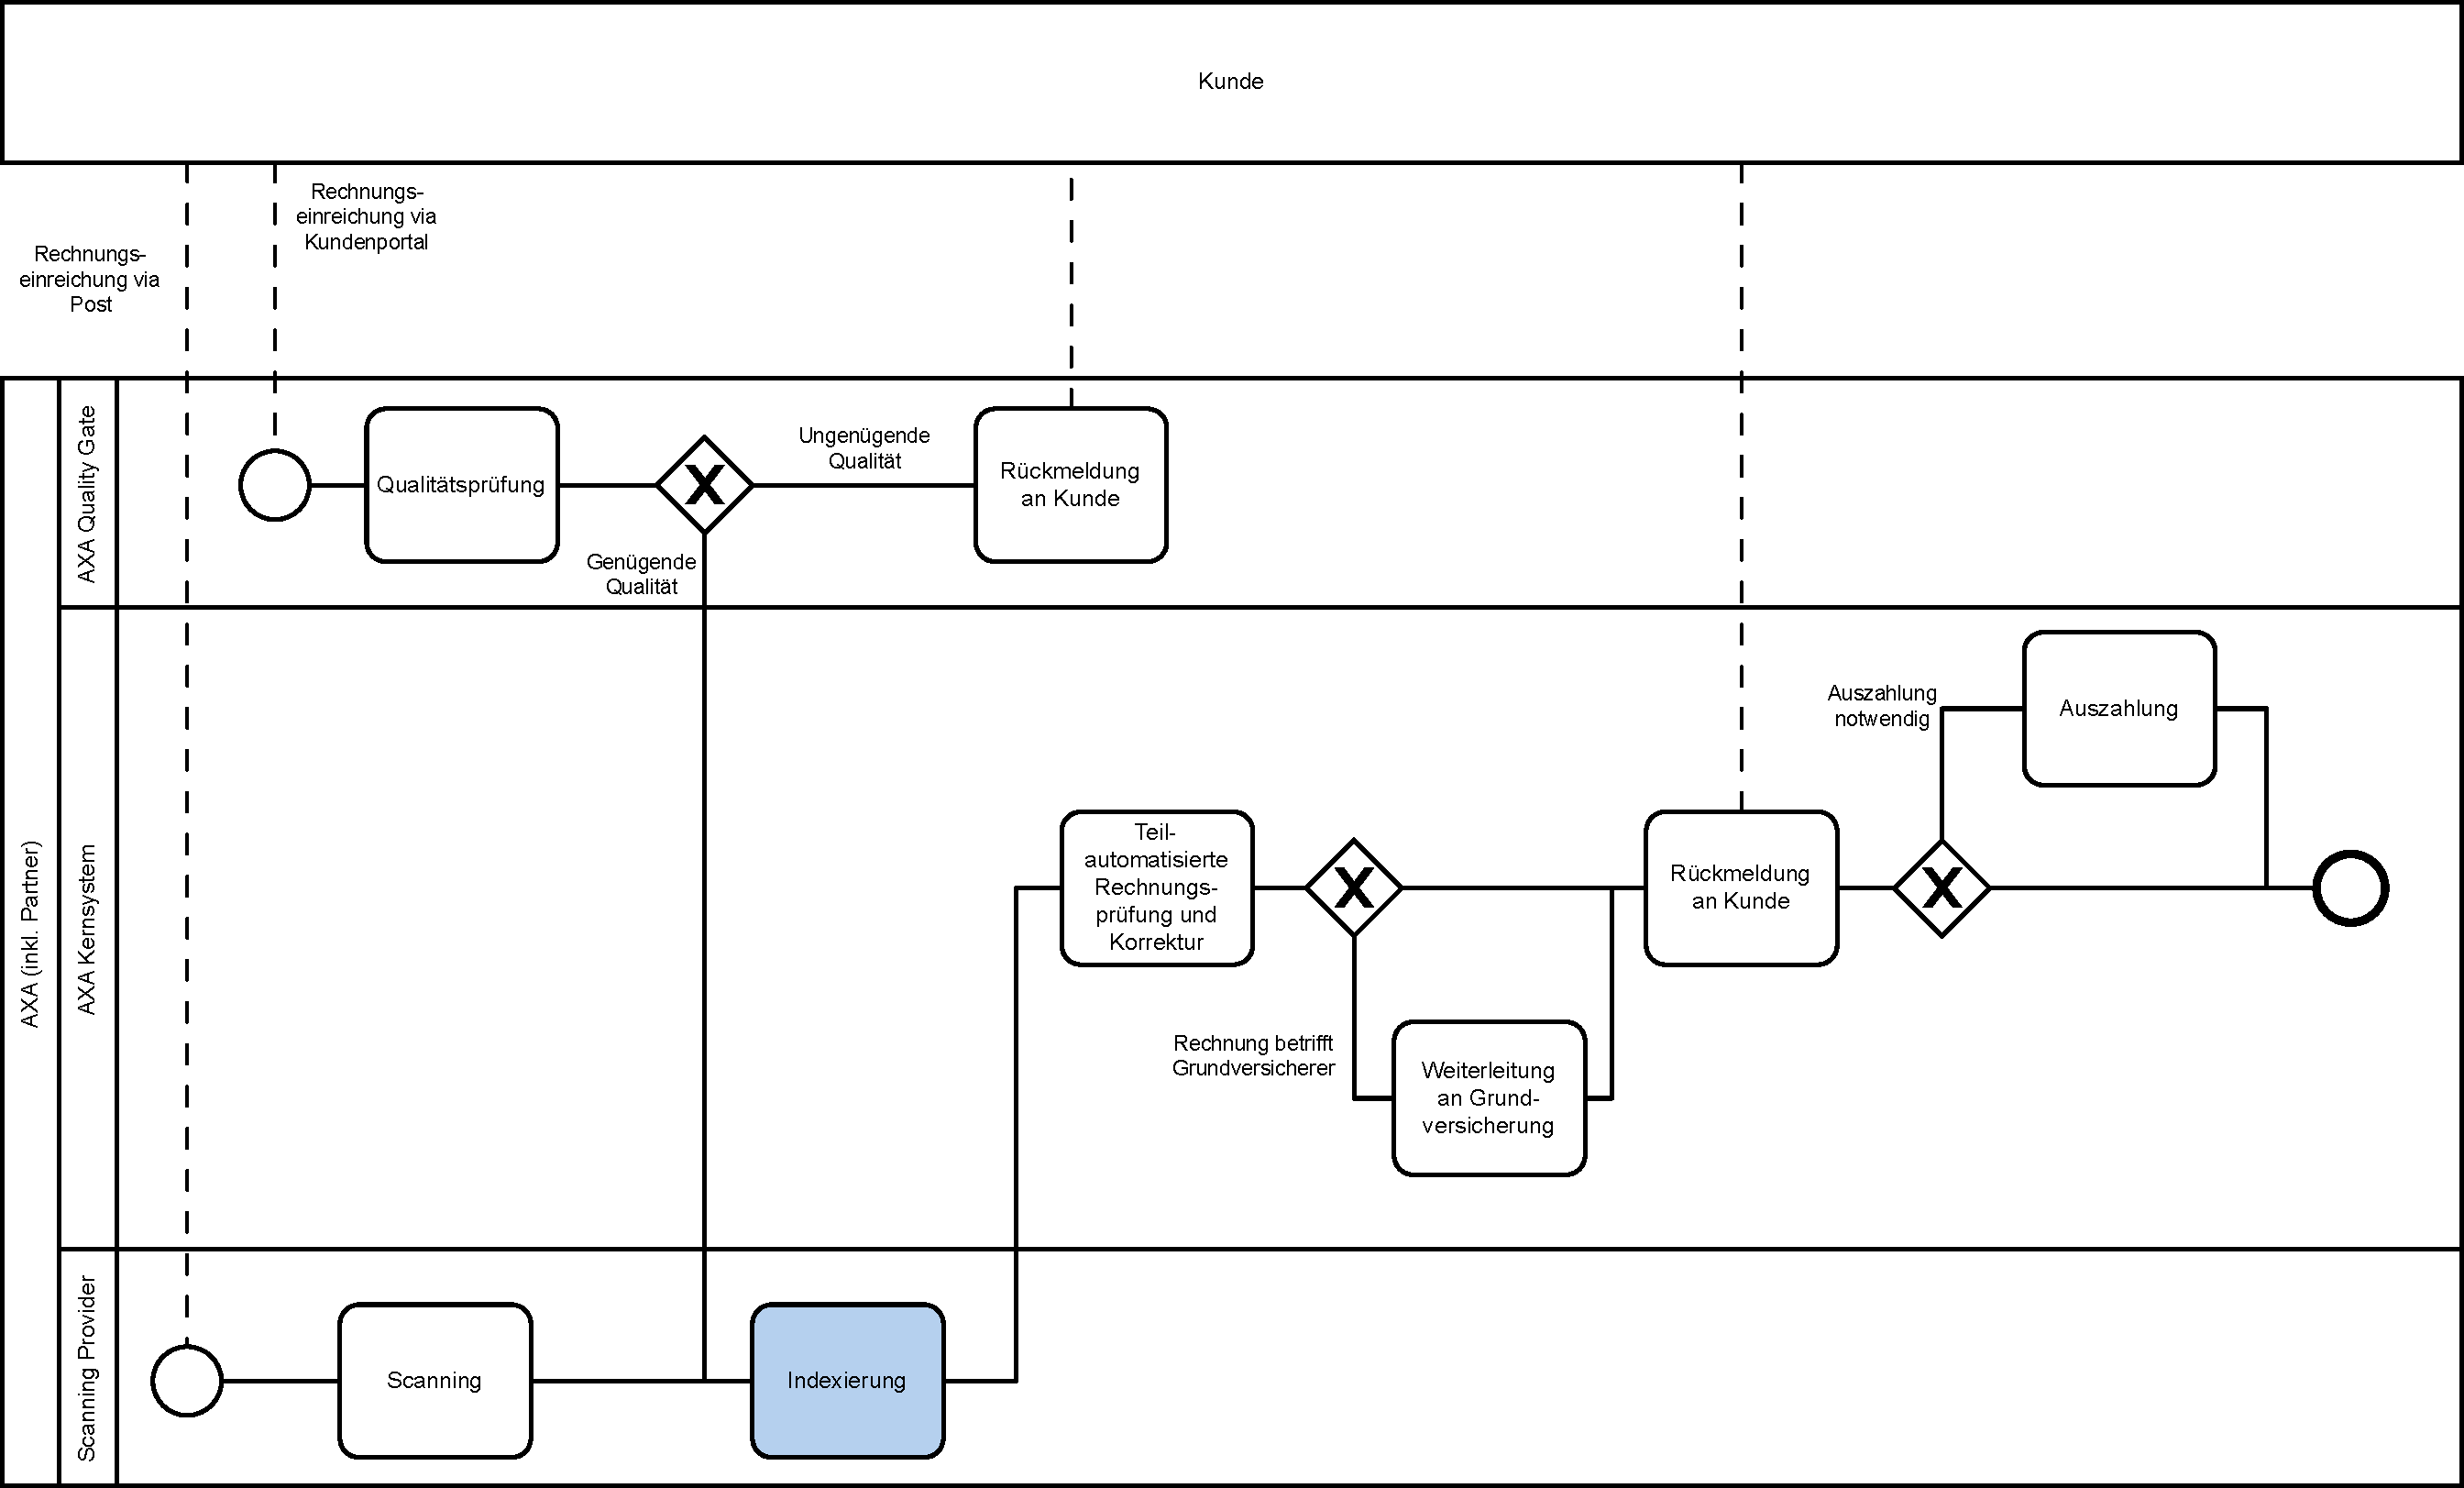
\includegraphics[width=\textwidth]{graphics/rechnungseinreichung-bpmn.pdf}
\end{figure}

\todo[inline]{Im BPMN Diagramm SVG export fehlen die Pfeile...}

Im Kundenportal hat der Kunde die Möglichkeit eine Rechnung hochzuladen. Dabei kann er entweder ein Dokument auf seinem Endgerät wählen oder die Kamera seines Geräts nutzen, um eine Rechnung zu fotografieren.

Nach erfolgreichem Hochladen der Rechnung im Kundenportal durchläuft diese eine erste manuelle Qualitätsprüfung. Diese Qualitätsprüfung wurde eingeführt, da hochgeladene Rechnung teilweise ungenügende Qualität vorweisen. Entspricht die Rechnung nicht den Qualitätsanforderungen oder fehlt eine Seite oder eine ärztliche Verordnung, so wird der Kunde gebeten, die vollständige Rechnung erneut hochzuladen.

Nach erfolgreicher Qualitätsprüfung wird die Rechnung an den Scanning und Indexierungsdienstleister der AXA weitergeleitet.

Entscheidet sich der Kunde für die Einreichung per Post, so wird sein Brief direkt an den Scanning und Indexierungsdienstleister der AXA weitergeleitet. Dieser Dienstleister scannt die weitergeleitete Rechnung ein.

Nach beiden dieser Einstiegspunkten in den Prozess indexiert nun der Scanning und Indexierungsdienstleister die eingereichte Rechnung. Dieser Aufgabenschritt erfolgt teilweise automatisiert und teilweise manuell. Wie genau die Indexierung abläuft ist nicht bekannt. Der genaue Ablauf dieser eingekauften Dienstleistung wird als Geschäftsgeheimnis gewahrt.

Nach der Indexierung werden die Scans sowie das strukturierte Resultat der Indexierung elektronisch an das Kernsystem der AXA Gesundheitsvorsorge übermittelt. Dieses Kern\-system verarbeitet die eingegangenen Rechnungen aufgrund eines Regelwerks. Kann die Rechnung nicht verarbeitet werden, weil diese nicht korrekt Indexiert wurde oder Informationen fehlen, muss eine FachspezialistIn eingreifen. Nach allfälligen Rückfragen und Korrekturen durch die FachspezialistIn wird die Rechnung verarbeitet. 

Nach der Erfolgreichen Verarbeitung der Rechnung wird der Kunde elektronisch informiert, ob die beanspruchten Leistungen versichert sind und ob eine Rückvergütung ausbezahlt wird.

Hat der Kunde die AXA bevollmächtigt, so wird die Rechnung in gewissen Fällen, je nach Rechnungspositionen, automatisiert an die Grundversicherung des Kunden weitergeleitet.

Ziel der AXA Gesundheitsvorsorge ist es, diesen Prozess für eingereichte Rechnungen, welche Fitnesscenter und Optiker betreffen, vollständig zu automatisieren. Dabei gibt es in diversen Bereichen Herausforderungen, welche aktuell angegangen werden. Diese Arbeit hat zum Ziel, die Herausforderungen im Bereich der Indexierung anzugehen. Es wird untersucht, ob die Anwendung künstlicher Intelligenz eine Automatisierung der Indexierung ermöglichen kann.

Ausgangslage für den Arbeitsschritt der Indexierung ist eine digitalisierte Rechnung. Ziel der Indexierung ist es, aus dieser Rechnung strukturierte Informationen zu gewinnen und an das Kernsystem der AXA zu übermittelt. In dieser Arbeit wird die Extraktion dieser strukturierten Daten aus den digitalisierten Rechnungen mit Hilfe künstlicher Intelligenz behandelt. Das Übermitteln der strukturierten Informationen an das Kernsystem ist bereits gelöst und aus diesem Grund kein Teil der Untersuchungen dieser Arbeit.

% Um den Umfang dieser Analyse einzugrenzen, wird der Fokus auf Rechnungen von Optikern, Fitnesscentern und Sportvereinen gelegt. Diese Rechnungen machen 23\% der eingereichten Rechnungen aus und sind Versicherungstechnisch relativ einfach handzuhaben.

% optiker 2660 -> 
% fitness 2055
% sportsclub 847
% =subtotla 5562
% other 18881
% =total 24443


\subsection{Anforderungen}

Um Rechnungen von Fitnesscenter und Optikern automatisiert verarbeiten zu können, müssen diese Rechnungen als solche klassifiziert und die notwendigen Informationen, welche nachfolgend genauer spezifiziert werden, extrahiert werden.

Um eine Rechnung eines Optikers zu verarbeiten, sind folgende Informationen relevant:

\begin{itemize}
    \item \textbf{Leistungsbezüger}
    
    Es muss ermittelt werden, für wen die Rechnung ausgestellt wurde. Anhand dieser Information wird geprüft, ob und wie diese Person bei der AXA versichert ist. Auch wird damit geprüft, dass der maximal versicherte Betrag noch nicht ausgeschöpft ist.
    
    Ist der Leistungsbezüger minderjährig, so wird ein gewisser Betrag von der Grundversicherung übernommen. In diesem Fall wird dieser Betrag von der Rückvergütung der AXA abgezogen und die Rechnung an die Grundversicherung weitergeleitet.
    
    \item \textbf{Totalbetrag der Rechnung (inkl. Währung)}
    
    Dieser Betrag bildet die Grundlage zur Berechnung der geschuldeten Leistung an den Kunden. 
    
    Einzelne Rechnungspositionen sind für Rechnungen von Optikern nicht relevant.
    
    \item \textbf{Hinweis auf eine ärztliche Verordnung}
    
    Besteht eine ärztliche Verordnung, ist ein gewisser Betrag bei der Grundversicherung versichert. In diesem Fall wird dieser Betrag von der Rückvergütung der AXA abgezogen und die Rechnung an die Grundversicherung weitergeleitet.
\end{itemize}

%\paragraph{
%    \textbf{Relevante Attribute einer Rechnung für einen Sportverein}
%}

%Eine Rechnung eines Sportvereins wird bei der AXA Anhand folgender Attribute beurteilt:

%\begin{itemize}
%    \item \textbf{Leistungsbezüger}
%    
%    Es muss ermittelt werden, für wen die Rechnung ausgestellt wurde. Anhand dieser Information wird geprüft ob und wie diese Person bei der AXA Versichert ist. Auch wird damit geprüft, dass der maximal versicherte Betrag noch nicht ausgeschöpft ist.
%    \item \textbf{Totalbetrag der Rechnung (inkl. Währung):}
%    
%    Dieser Betrag bildet die Grundlage zur Berechung des geschuldeten Betrages. 
%    
%    Einzelne Rechnungspoisition sind für Rechnungen eines Sportvereins nicht relevant.
%    \item \textbf{Sportart}
%    
%    Die AXA anerkennt alle olympischen Sportarten. Das bedeutet, gewisse Sportarten sind nicht versichert. Es muss also die Sportart ermittelt werden, um die Versicherungsdeckung zu prüfen.
%\end{itemize}

Folgende Informationen sind notwendig, um eine Rechnung für ein Fitness-Abo zu verarbeiten:

\begin{itemize}
    \item \textbf{Leistungsbezüger}
    
    Es muss ermittelt werden, für wen die Rechnung ausgestellt wurde. Anhand dieser Information wird geprüft ob und wie diese Person bei der AXA versichert ist. Auch wird damit geprüft, dass der maximal versicherte Betrag noch nicht ausgeschöpft ist.
    \item \textbf{Totalbetrag der Rechnung (inkl. Währung):}
    
    Dieser Betrag bildet die Grundlage zur Berechnung der geschuldeten Leistung an den Kunden. 
    
    Einzelne Rechnungspositionen sind für Rechnungen von Optikern nicht relevant.
    \item \textbf{Fitnesscenter (Leistungserbringer)}
    
    Die AXA anerkennt alle Fitnesscenter mit dem Label Qualitop von Qualicert oder mit einer Bewertung von mindestens 3 Sternen bei Fitnessguide.
\end{itemize}

Anhand dieser Informationen können Rechnungen automatisiert verarbeitet werden. Es ist wichtig, dass diese Informationen korrekt extrahiert werden, denn durch die Automatisierung entfällt jegliche manuelle Prüfung. Fehler würden, wenn überhaupt, erst dem Kunden auffallen. 

\todo[inline]{Sollen hier bereits hard requirements (e.g. wieviele Rechnungen dürfen falsch indexiert werden) aufgestellt werden?}

\subsection{Vorgehen und Methodik}

Wie in den Anforderungen an die Indexierung bereits angemerkt, müssen zwei Teilschritte, die Klassifizierung und die Extraktion von Informationen, analysiert werden. Für beide diese Teilschritte wird je ein separates Experiment durchgeführt. Der Ablauf der Experimente ist dabei identisch. 

Für beide Experimente werden zuerst Testdaten aus dem System der AXA extrahiert und aufbereitet. Für die beiden Experimente werden jeweils eine oder mehrere künstliche Intelligenzen geschaffen. Die Resultate der beiden Experimente werden jeweils unabhängig voneinander diskutiert.

Aus den Diskussionen der beiden Experimente werden Schlussfolgerungen für die Anwendbarkeit der künstlichen Intelligenz zur Indexierung von Rechnungen abgeleitet. Neben dem Erfolg der Experimente werden dabei auch das Potential der gewählten Ansätze sowie mögliche weitere Ansätze diskutiert.



